\begin{frame}{¿Cómo viabilizar las reformas?}
\begin{itemize}
    \item En el prefacio del libro escribo: \textit{``Un manejo fiscal responsable contribuye a mantener tasas de interés más bajas, creando un entorno favorable para la inversión privada, la generación de empleo y el crecimiento económico''}.
    \item Pero en un país donde el votante medio es \textbf{autoempleado} y no tiene acceso al \textbf{crédito formal}, este argumento probablemente \textbf{no} resulta convincente.
    \item Menos aún si el ajuste se asocia con medidas como reducir el acceso a servicios de salud o gravar con IVA la canasta familiar.
    \item En ese escenario, será natural que mucha gente pregunte por qué los acreedores no deben asumir al menos parte del ajuste.
    \item ¿Hace esto políticamente inviable un ajuste fiscal?
\end{itemize}
\end{frame}

%\section{¿Qué sigue ahora?}

%\begin{frame}{¿Qué sigue ahora?}
\begin{frame}{¿Cómo viabilizar las reformas?}
    \begin{figure}
        \centering
        
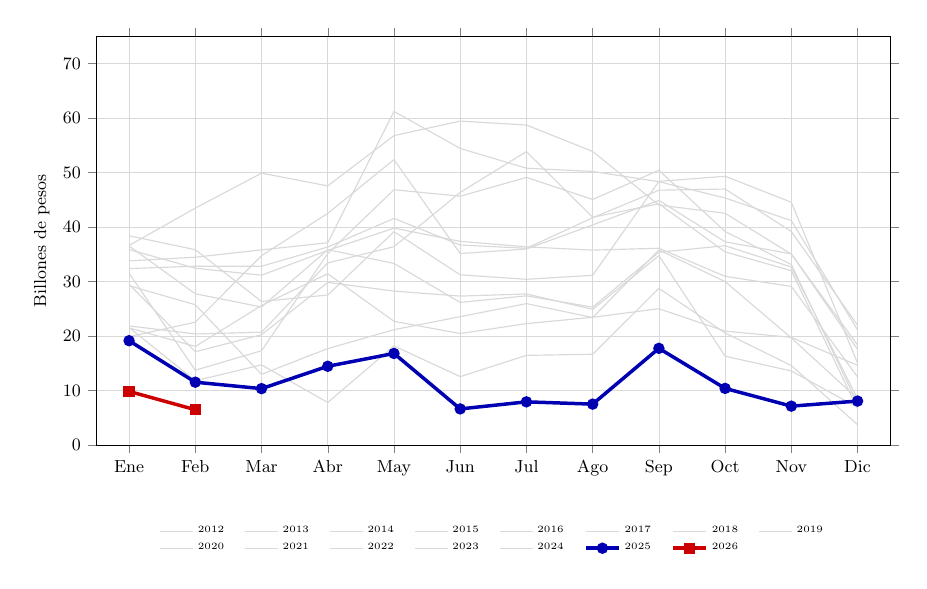
\begin{tikzpicture}[scale=0.7]
\begin{axis}[
    width=16cm,
    height=9cm,
    xlabel={},
    ylabel={Billones de pesos},
    xmin=0.5, xmax=12.5,
    ymin=0, ymax=75,
    xtick={1,2,3,4,5,6,7,8,9,10,11,12},
    xticklabels={Ene,Feb,Mar,Abr,May,Jun,Jul,Ago,Sep,Oct,Nov,Dic},
    ytick={0,10,20,30,40,50,60,70},
    yticklabel={\pgfmathprintnumber[fixed,precision=0]{\tick}},
    y tick label style={/pgf/number format/1000 sep={.}},
    grid=both,
    grid style={line width=0.3pt, draw=gray!20},
    major grid style={line width=0.4pt, draw=gray!30},
    tick align=outside,
    tick label style={font=\small},
    label style={font=\small},
    legend style={
        at={(0.5,-0.18)},
        anchor=north,
        legend columns=8,
        font=\tiny,
        draw=none,
        /tikz/every even column/.append style={column sep=0.3cm}
    },
    legend cell align=left,
    clip=false,
]

% ---- años en gris tenue (2012-2024) ----
\def\graycol{gray!35}

% 2012
\addplot[color=gray!30, line width=0.6pt, mark=none]
coordinates {(1,21.847)(2,20.369)(3,20.691)(4,33.401)(5,36.384)(6,46.334)(7,53.822)(8,41.780)(9,44.248)(10,35.422)(11,31.977)(12,6.632)};
\addlegendentry{2012}

% 2013
\addplot[color=gray!30, line width=0.6pt, mark=none]
coordinates {(1,29.222)(2,25.729)(3,12.964)(4,17.694)(5,21.153)(6,23.543)(7,25.937)(8,23.383)(9,35.769)(10,29.975)(11,19.643)(12,8.487)};
\addlegendentry{2013}

% 2014
\addplot[color=gray!30, line width=0.6pt, mark=none]
coordinates {(1,21.481)(2,18.072)(3,25.599)(4,31.407)(5,22.688)(6,20.450)(7,22.267)(8,23.434)(9,24.999)(10,20.893)(11,19.742)(12,14.616)};
\addlegendentry{2014}

% 2015
\addplot[color=gray!30, line width=0.6pt, mark=none]
coordinates {(1,29.499)(2,17.112)(3,20.233)(4,29.825)(5,28.235)(6,27.315)(7,27.709)(8,24.892)(9,34.735)(10,16.298)(11,13.583)(12,6.903)};
\addlegendentry{2015}

% 2016
\addplot[color=gray!30, line width=0.6pt, mark=none]
coordinates {(1,19.865)(2,22.541)(3,34.733)(4,42.487)(5,52.353)(6,35.118)(7,35.953)(8,40.376)(9,44.865)(10,37.275)(11,35.059)(12,17.554)};
\addlegendentry{2016}

% 2017
\addplot[color=gray!30, line width=0.6pt, mark=none]
coordinates {(1,32.369)(2,32.793)(3,32.785)(4,36.325)(5,41.565)(6,36.687)(7,36.084)(8,41.695)(9,46.739)(10,46.951)(11,39.154)(12,21.977)};
\addlegendentry{2017}

% 2018
\addplot[color=gray!30, line width=0.6pt, mark=none]
coordinates {(1,35.860)(2,32.427)(3,31.149)(4,35.701)(5,39.780)(6,37.357)(7,36.353)(8,35.748)(9,36.093)(10,30.942)(11,29.088)(12,12.482)};
\addlegendentry{2018}

% 2019
\addplot[color=gray!30, line width=0.6pt, mark=none]
coordinates {(1,36.600)(2,43.451)(3,49.867)(4,47.532)(5,56.753)(6,59.414)(7,58.692)(8,53.850)(9,44.011)(10,42.506)(11,35.007)(12,18.348)};
\addlegendentry{2019}

% 2020
\addplot[color=gray!30, line width=0.6pt, mark=none]
coordinates {(1,33.783)(2,34.446)(3,35.795)(4,37.101)(5,61.192)(6,54.401)(7,50.774)(8,50.178)(9,48.300)(10,45.313)(11,41.160)(12,21.118)};
\addlegendentry{2020}

% 2021
\addplot[color=gray!30, line width=0.6pt, mark=none]
coordinates {(1,38.380)(2,35.828)(3,26.331)(4,27.513)(5,39.136)(6,31.217)(7,30.398)(8,31.131)(9,48.355)(10,49.297)(11,44.531)(12,15.013)};
\addlegendentry{2021}

% 2022
\addplot[color=gray!30, line width=0.6pt, mark=none]
coordinates {(1,36.515)(2,27.739)(3,25.314)(4,35.832)(5,33.304)(6,26.155)(7,27.366)(8,25.285)(9,35.361)(10,36.558)(11,32.652)(12,8.467)};
\addlegendentry{2022}

% 2023
\addplot[color=gray!30, line width=0.6pt, mark=none]
coordinates {(1,31.518)(2,13.720)(3,17.294)(4,35.125)(5,46.828)(6,45.635)(7,49.088)(8,45.037)(9,50.398)(10,39.165)(11,33.092)(12,7.586)};
\addlegendentry{2023}

% 2024
\addplot[color=gray!30, line width=0.6pt, mark=none]
coordinates {(1,21.549)(2,11.789)(3,14.695)(4,7.801)(5,18.180)(6,12.544)(7,16.444)(8,16.648)(9,28.744)(10,20.548)(11,14.575)(12,3.727)};
\addlegendentry{2024}

% ---- 2025: azul oscuro ----
\addplot[color=blue!70!black, line width=1.8pt, mark=*, mark size=2pt]
coordinates {(1,19.133)(2,11.524)(3,10.344)(4,14.443)(5,16.795)(6,6.622)(7,7.920)(8,7.501)(9,17.735)(10,10.385)(11,7.131)(12,8.061)};
\addlegendentry{2025}

% ---- 2026: rojo ----
\addplot[color=red!80!black, line width=1.8pt, mark=square*, mark size=2pt]
coordinates {(1,9.834)(2,6.474)};
\addlegendentry{2026}

\end{axis}
\end{tikzpicture}

        \caption{Depósitos del Tesoro Nacional - Pesos Constantes de Febrero de 2026}
        \label{fig:despositos}
    \end{figure}
\end{frame}


\begin{frame}{¿Cómo viabilizar las reformas?}
    \begin{itemize}
        \item La necesidad de ajuste aumentará a medida que se estrechen las condiciones de liquidez.
        \item Mientras el mercado continúe financiando al Gobierno, el ajuste podrá seguir aplazándose.
        \item Pero si se interrumpe el acceso al financiamiento, la \textbf{restricción de liquidez} terminará forzándolo.
    \end{itemize}
\end{frame}

\begin{frame}{¿Cómo viabilizar las reformas?}
    \begin{itemize}
        \item En ese escenario, la crisis de caja se traducirá en \textbf{recortes abruptos}, \textbf{congelamiento de apropiaciones} y \textbf{atrasos en pagos}, con riesgo incluso para el \textbf{servicio de la deuda}.
        \item El Gobierno podría obtener liquidez transitoria recurriendo a \textbf{organismos multilaterales}, que probablemente condicionarían su apoyo a un \textbf{paquete de ajuste}.
        \item Si las presiones de liquidez se agravan y el acceso al financiamiento se cierra de forma persistente, tampoco puede descartarse una \textbf{reestructuración de la deuda}.
    \end{itemize}
\end{frame}


\begin{comment}
\begin{frame}{¿Cómo viabilizar las reformas?}
\begin{itemize}
    \item En otras palabras, un equilibrio político en el que la inversión, el empleo y el crecimiento se mantienen deprimidos (\textit{debt overhang}) puede parecer más viable que un ajuste fiscal explícito.
    \item No obstante, el ajuste llegará tarde o temprano: de manera ordenada, o por las \textbf{restricciones de liquidez} que enfrentará el Gobierno si se cierra el financiamiento.
    \item En ese momento, muchos ciudadanos se preguntarán por qué el ajuste no recae también sobre los \textbf{acreedores}.
\end{itemize}
\end{frame}

\begin{frame}{¿Cómo viabilizar las reformas?}
\begin{itemize}
    \item En el caso de la deuda interna, los principales acreedores son los fondos de pensiones, los bancos y las aseguradoras.
    \item Por eso, no se puede descartar que el debate termine desplazándose hacia las consecuencias financieras de una eventual reestructuración de la deuda.
\end{itemize}
\end{frame}

\begin{frame}{¿Qué sigue ahora?}
\begin{itemize}
    \item Si la consolidación fiscal se ve tan difícil, ¿por qué los inversionistas continúan financiando al Gobierno?
    \begin{itemize}
        \item ¿Confía el mercado en que el próximo Gobierno sí hará el ajuste?
        \item ¿Hay inversionistas apostándole a salir antes de un cambio brusco en las condiciones financieras?
        \item ¿Cree el mercado que el ajuste llegará por iliquidez antes que por decisión política?
        \item ¿Hay una apuesta implícita a un rescate o a una refinanciación con organismos multilaterales a cambio de anunciar un paquete de medidas?
    \end{itemize}
\end{itemize}
\end{frame}
\end{comment}